% Teaser for the paper (Case Study 2): the ParaView image, the box spec and a provenance
% excerpt, as one standalone figure 7 in wide (the VGTC conference text width).
% Overleaf: upload this file with teaser_paraview.png and compile with pdfLaTeX; then
% 
\includegraphics[width=\linewidth]{teaser} in the paper's \teaser{...}.
% Locally: latexmk -pdf teaser.tex; pdftoppm -r 300 -png -singlefile teaser.pdf teaser
% The image is built by ../scripts/teaser_background.py from animation.0044.png.
\documentclass[9pt]{article}
\usepackage[paperwidth=7in, paperheight=2.6in, margin=0pt]{geometry}
\usepackage{times}
\renewcommand*\ttdefault{txtt}
\usepackage{graphicx}
\usepackage{listings}
\usepackage{xcolor}
\pagestyle{empty}
\setlength{\parindent}{0pt}
% The spec is the larger of the two listings: the reader's eye goes there first.
\newcommand{\specsize}{\fontsize{8}{9.5}\selectfont}
\newcommand{\provsize}{\fontsize{6.8}{8}\selectfont}
\lstset{breaklines=false, columns=fullflexible, keepspaces=true, numbers=none,
        frame=tb, framerule=0.4pt, showstringspaces=false,
        aboveskip=0pt, belowskip=0pt, framesep=3pt}

\begin{document}
\vspace*{\fill}
\begin{minipage}[c]{0.56\textwidth}
  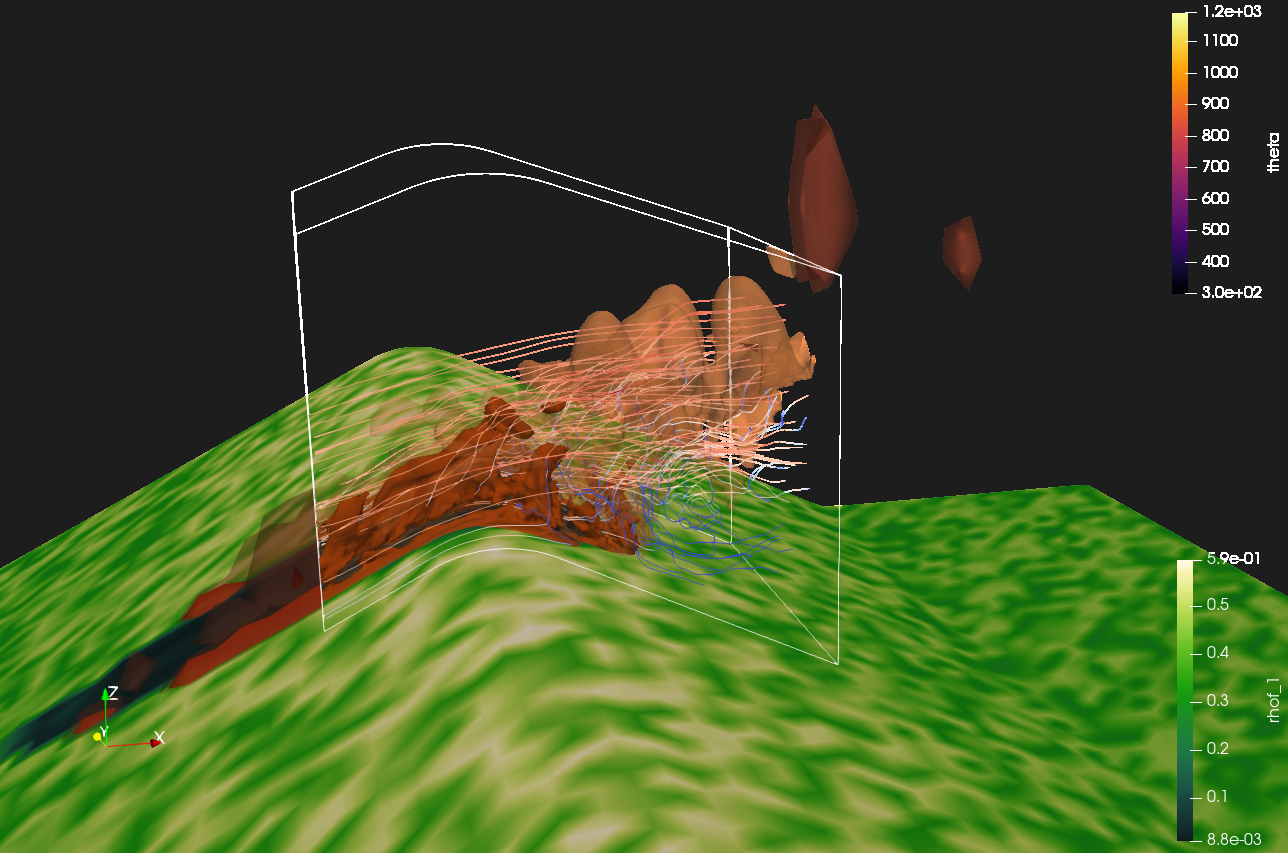
\includegraphics[width=\linewidth]{teaser_paraview}
\end{minipage}\hfill
\begin{minipage}[c]{0.42\textwidth}
\begin{lstlisting}[language=Python, basicstyle=\ttfamily\specsize]
src  = source("ssh://host/wildfire/")
view = timesteps(src, 9000, 45000)
view = fields(view, ["theta", "u", "v", "w"])
view = region(view, x=(-100, 200), y=(-120, 120),
              z=(0, 350), coords="world")
save(view, "box.vts")
\end{lstlisting}
\vspace{12pt}
\begin{lstlisting}[basicstyle=\ttfamily\provsize\color{black!75}]
# from the provenance record in each output
Steps
  1. timesteps  keep timesteps #9000 to #45000
  2. fields     keep theta, u, v, w; drop O2, ...
  3. region     keep the samples inside the box
                (world coordinates), placed on
                the file's geometry
  4. save       write one VTK StructuredGrid file
                per timestep: each point at its
                own position from the source
\end{lstlisting}
\end{minipage}
\vspace*{\fill}
\end{document}
